%------------------------------------------------------------------------------
% Template file for the submission of papers to IUCr journals in LaTeX2e
% using the iucr document class
% Copyright 1999-2013 International Union of Crystallography
% Version 1.6 (28 March 2013)
%------------------------------------------------------------------------------

%\documentclass[preprint]{iucr}              % DO NOT DELETE THIS LINE
\documentclass{iucr}              % DO NOT DELETE THIS LINE

\usepackage{siunitx}
\usepackage{color}
\usepackage{amsmath,amssymb}
\usepackage{mathtools}
\usepackage[normalem]{ulem}

\newcommand{\todo}[1]{{\color{red}[TODO: "#1'']}}
\newcommand{\inblue}[1]{{\color{blue}#1}}
\newcommand{\inred}[1]{{\color{red}#1}}
\newcommand{\ingreen}[1]{{\color{green}#1}}
\newcommand{\soutred}[1]{{\color{red}\sout{#1}}}


     %-------------------------------------------------------------------------
     % Information about journal to which submitted
     %-------------------------------------------------------------------------
     \journalcode{S}              % Indicate the journal to which submitted
                                  %   A - Acta Crystallographica Section A
                                  %   B - Acta Crystallographica Section B
                                  %   C - Acta Crystallographica Section C
                                  %   D - Acta Crystallographica Section D
                                  %   E - Acta Crystallographica Section E
                                  %   F - Acta Crystallographica Section F
                                  %   J - Journal of Applied Crystallography
                                  %   M - IUCrJ
                                  %   S - Journal of Synchrotron Radiation

\begin{document}                  % DO NOT DELETE THIS LINE

     %-------------------------------------------------------------------------
     % The introductory (header) part of the paper
     %-------------------------------------------------------------------------

     % The title of the paper. Use \shorttitle to indicate an abbreviated title
     % for use in running heads (you will need to uncomment it).

\title{Wofry for Optics}
%\shorttitle{Short Title}

     % Authors' names and addresses. Use \cauthor for the main (contact) author.
     % Use \author for all other authors. Use \aff for authors' affiliations.
     % Use lower-case letters in square brackets to link authors to their
     % affiliations; if there is only one affiliation address, remove the [a].

\cauthor[a]{Manuel}{Sanchez del Rio}{srio@esrf.eu}{address if different from \aff}
\author[b]{Luca}{Rebuffi}


\aff[a]{European Synchrotron Radiation Facility, 71 Avenue des Martyrs, 38000 Grenoble \country{France}}
% \aff[b]{Second affiliation address}

     % Use \shortauthor to indicate an abbreviated author list for use in
     % running heads (you will need to uncomment it).

%\shortauthor{Soape, Author and Doe}

     % Use \vita if required to give biographical details (for authors of
     % invited review papers only). Uncomment it.

%\vita{Author's biography}

     % Keywords (required for Journal of Synchrotron Radiation only)
     % Use the \keyword macro for each word or phrase, e.g. 
     % \keyword{X-ray diffraction}\keyword{muscle}

%\keyword{infrared beamline}

     % PDB and NDB reference codes for structures referenced in the article and
     % deposited with the Protein Data Bank and Nucleic Acids Database (Acta
     % Crystallographica Section D). Repeat for each separate structure e.g
     % \PDBref[dethiobiotin synthetase]{1byi} \NDBref[d(G$_4$CGC$_4$)]{ad0002}

%\PDBref[optional name]{refcode}
%\NDBref[optional name]{refcode}

\maketitle                        % DO NOT DELETE THIS LINE

\begin{synopsis}
Wofry 1D, a newly developed tool of undulator radiation coherent mode decomposition in 1D.
\end{synopsis}

\begin{abstract}
We used a new software tool to perform coherent mode decomposition of the undulator radiation in 1D.  
\end{abstract}


     %-------------------------------------------------------------------------
     % The main body of the paper
     %-------------------------------------------------------------------------
     % Now enter the text of the document in multiple \section's, \subsection's
     % and \subsubsection's as required.

\section{Introduction}


xxx

The paper is organized as follows. Section 2 summarizes the methodology used for 1D coherent mode decomposition of undulator beams. Section 3 analyzes the focusing of partially coherent beams with a single refractive system (lens). Section 4 discusses the pairing of two refractive systems. Section 5 shows simulations for the full beamline and compares different methodologies for a selected case. A general discussion is in section 6 and concluding remarks in section 7. 

\section{One dimensional coherent mode decomposition of an undulator source and propagation along a beamline with lenses}

For the calculations presented in this paper we have developed a new tool for dealing with partially coherence beams produced by undulators in low-emittance storage rings. For that, we developed a 1D model of the coherent mode decomposition previously developed in 2D \cite{glass2017}. The motivation for developing these new tools is to perform quick calculations (e.g., being able to perform parametric calculations in a laptop) with high accuracy in the simulation of the source and beam propagation. We believe that the separation of the real 2D wavefront in two separated 1D wavefronts is well justified for most synchrotron beamlines, where the cross-talk between these two directions is small. 
The tools developed here are included in the OASYS toolbox \cite{codeOASYS}, available in the WOFRY add-on \cite{XX}. These tools are completely scriptable so they can be used from the OASYS interface, which also creates scripts that can be a posteriori modified for batch runs. 

\subsection{Partial coherence modeling the undulator beam using coherent mode decomposition}

The electrons in an storage ring are statistically distributed, following (in good approximation) a Gaussian distribution in a 6-dimensional space (three spatial coordinates, two angles to define direction, and the electron energy). Many electrons therefore contribute to photon beam radiation, each one creating a wavefront. The consequence is that the overall radiation cannot be described deterministically which implies that statistical methods are needed, like for describing the electron beam. This is the origin of partial coherence of the synchrotron emission. As stated before, in an ideal storage ring of zero emittance, the electrons follow a filament beam so the emission is fully coherent. As soon as  electron emittance increases, the electrons contributing to the radiation start to have different initial conditions (in the 6-dimensional space) and the overall emission cannot be describe by a single wavefront, but by statistically distributed wavefronts, described by partial coherent optics.

Under some approximations the radiation is 'wide sense stationary' \cite{mandel_wolf}. These conditions are satisfied for light emitted by storage rings (but not for XFELs) \cite{geloni2008}, and can be summarized in
i) the electron bunch length is long enough,
ii) radiation is monochromatized 'not too much' (like by standard monochromators), and 
iii) the radiation frequency is large enough.
It is in this case all the coherent properties of the radiation can be described using the 'cross spectral density' (CSD), a complex function that measures the correlation of the electric field in two different spatial points at a given radiation frequency. It can be mapped in a $(x,y)$ plane at a third coordinate $z$. At that plane, the CSD depends on 5 variables: 

\begin{equation}
W_{2D}(x_1,y_1,x_2,y_2;\omega) = <E^*(x_1,y_1;\omega) E(x_2,y_2;\omega)>
\label{eq:CSD_1D}
\end{equation}

In the following, we suppose that the CSD is separable in its 1D horizontal $x$ and vertical $y$ coordinates, therefore the $W_{2D}$ becomes a product of two CSD functions $W$ of two variables for a given photon frequency $\omega$:

\begin{equation}
W_{2D}(x_1,y_1,x_2,y_2;\omega) = W(x_1,x_2;\omega) W(y_1,y_2;\omega).
\label{eq:CSD_2D}
\end{equation}
Each $W$ function is treated separately in a similar way affecting the $x$ (horizontal) and $y$ (vertical) coordinate.

From the cross spectral density one can calculate the 'spectral density' (usually simply called 'intensity') $I(x;\omega)=W(x,x,\omega)$, and also the complex degree of (transverse) coherence: 
\begin{equation}
\mu(x_1,x_2;\omega) = \frac{W(x_1,x_2;\omega)}{\sqrt{I(x_1;\omega)}\sqrt{I(x_2;\omega)}}
\label{eq:DTC}
\end{equation}
The modulus of the complex degree of coherence is one for a completely coherent beam and zero for an incoherent beam. 

An important result in partial coherence optics permits to describe the radiation as an infinite sum of independent coherent modes (in the sense of orthonormality) :

\begin{equation}
W(x_1,x_2;\omega) = \sum_{n=0}^{\infty} \lambda_n(\omega) \Phi_n^*(x_1;\omega) \Phi_n(x_2;\omega) 
\label{eq:CMD}
\end{equation}
where $\lambda_n$ (eigenvalues) are the intensity weights and the $\Phi_n$ are the coherent modes (eigenfunctions). 
Some important characteristics of this coherent mode decomposition are: i) the modes are orthonormal (in the integral sense), ii) the modes maximize the spectral density, the first mode is more intense than the second, and so on, meaning that the truncated expansion is optimal, and iii) there is complete coherence if and only if there is only a single mode. If one can truncate the infinite series to a limited number of modes $N$ which contain a good percentage of the spectral density, the numerical storage of the $N$ modes that depend on two spatial variables is usually more economic than the storage of the cross spectral density $W$ that depends on four variables. 
The eigenvalues $\lambda_n$ are a measure of the intensity. Indeed, one can define the occupation $\eta$ of the i-th mode as the ratio of its intensity to the total intensity: 

\begin{equation}
\eta_i(\omega) = \frac{\lambda_i(\omega)}{\sum_{n=0}^{\infty} \lambda_n(\omega)}
\end{equation}

From these arguments, it is now natural to rigorously define Coherent Fraction ($CF$) as the occupation of the first coherent mode: $CF=\eta_0$.

The eigenvalues and the coherent modes are obtained by performing the Coherent mode decomposition (CMD). They are solution of the homogeneous Fredholm integral equation of second kind \cite{glass2017}. This is an eigenvalue problem. The numerical solution is obtained from the diagonalization of the CSD, which is a multivariate tensor when sampled at the point coordinates. This diagonalization problem is solved in 2D (i.e., $W_{2D}$ is a function of 4 variables) using complex numerical algorithms implemented in COMSYL. Fortunately, in 1D, the CSD is a function of two variables, represented in a matrix that can be easily diagonalized using standard tools availables in python-numpy. The numerical calculation of $W(x_1,x_2)$ uses Kim's convolution theorem \cite{kim1986b} as described in \cite{glass2017}. It includes two ingredients: i) the statistical parameters of the electron beam at the undulator center (sizes and divergences), and ii) the intensity distribution of the undulator emission at the undulator center. The undulator emission is calculated in a plane far enough from the undulator using classical electrodynamics \cite{jackson} (as implemented in the pySRU python library \cite{pySRU}), and then backpropagated (using a Fresnel propagator) to the center of the undulator. 

It is important to calculate the real emission of the undulator which is very different than a Gaussian. However, the (inadequate) use of a Gaussian approximation for the undulator radiation is often found in literature, e.g.  \cite{coisson1997}. In this case the Kim convolution predicts a CSD that is identical to the Gaussian Shell-method (GSM). Parameters of the undulator approximated by a GSM can be calculating by matching the coherent as explained in Appendix \ref{appendix:matchCF}). There is another argument in favour of using non-approximated coherent modes: small differences in a mode in terms of shape (even maintaining the same FWHM) may give to completely different results after propagation. Moreover, the GSM modes are real functions (constant phase) whereas the modes from CMD of undulator sources are complex functions (with a non-constant phase).

The interest of the coherent mode decomposition method is twofold: the possibility to propagate a partial coherent beam along the beamline by just propagating a few modes (less modes for a more coherent beam) which behave like coherent wavefronts, and the use of the coherent fraction (a scalar parameter) as a accurate well-defined measure of how coherent is the beam at any position of the beamline.

\subsection{Wavefront propagation}

% In the limiting case of zero emittance (i.e., ``single-electron" or filament beam), the undulator emission is fully coherent and the wavefront can be calculated using the classical electrodynamics \cite{XX}. These equations are implemented in the pySRU python library \cite{XX} that is used to calculate the undulator emission at a given distance from the source. 

The wavefront evolves when transported in free space from two different positions along the optical axis. We used integral propagators to calculate the wavefront in a given point using the wavefront in another position. In wofry we implemented two propagators, one based on the direct implementation of the  Rayleigh-Sommerfeld integral, and a second one, the zoom propagator, is a Fresnel propagator using FFT. Both propagators are described in \cite{srioLBL}. The effect of the different elements needed for the simulations in this work are presented in the following sections. 


\subsection{Wavefront modification by apertures}

A generic aperture is a mask that transmits a part of the wavefront in a range $[x_{min},x_{max}]$ and absorbs the rest. It can be
\begin{equation}
R(x;\omega) =
\left\{
\begin{matrix}
A,  & \mbox{~~if~~} x_{min} \le x \le x_{max}
\\ 
1 - A, & \mbox{~~elsewhere}
\end{matrix}
\right.
\end{equation}
When the element is a slit, then $A=1$. If it is a beamstop, then $A=0$. In the following simulations we will use an aperture of finite length $a$ centered with the beam, therefore $x_{min}=-a/2$ and $x_{max}=a/2$.

A sometimes useful case is the ``Gaussian slit" where $A=\exp(-x^2/(2\sigma_a))$. \todo{check is Gaussian applies to amplitude or intensity (in that case is divided by 4 instead 2)} The aperture acts as a Gaussian appodization window. Although artificial, it is interesting to shape the beam with a Gaussian profile, which remains a Gaussian after propagation. Therefore, a Gaussian slit acting on a plane wavefront does not produce diffraction fringes. Several recipes are proposed to relate $\sigma_a$ with the slit aperture $a=x_{max}-x_{min}$. We found convenient to define $\sigma_a=\Delta a/2.355$ (see Appendix \ref{appendix:slit}).

\subsection{Wavefront modification by refractive systems}

\subsubsection{Ideal lens}
We can define an ideal lens as a focusing device that converts a plane wave into a spherical wave collapsing to the focus at a distance $f$ from the ideal lens position. Therefore
\begin{equation}
    R(x;\omega) = e^{-i k~x^2/(2 f)}.
\end{equation}

An ideal coupling of $N$ ideal lenses will present a focal length $f=(f_1^{-1}+f_2^{-1}+...+f_N^{-1})^{-1}$. 

\subsubsection{Thin object} A refractor made by a material with refraction index $n(\omega)=1-\delta(\omega)+i\beta(\omega)$ 
%($n$ depends the photon wavelength $\lambda$)
and thickness profile $z(x)$ adds a phase to the wavefront $-\lambda \delta(\omega) z(x)$ and reduce its amplitude by $\exp(-\mu z(x)/2)$, where $\mu=(4 \pi/\lambda) \delta(\omega)$ is the (intensity) attenuation coefficient and $\lambda$ the photon wavelength. These expressions can be applied to any transmission object of profile $x(z)$ assuming valid the thin object approximation. 


\subsubsection{Real lens} The changes induced by a real lens in the wavefront can be calculated using the thin object approximation discussed below, using the lens profile. Usually, a single lens has a parabolic profile $z=x^2/(4R)$ with $R$ the radius the apex. A lens has two parabolic profiles (front and back) separated by a lens thickness $d$ and a flat profile outside the lens aperture $L$, therefore:
\begin{align}
    z(x) &= \frac{1}{2R} z^2 + d; & x < L/2\\ \nonumber
    z(x) &= \frac{1}{2R} (L/2)^2 + d; & x \ge L/2.
\end{align}

\subsubsection{CRLs and transfocators}
A Compound Refractive Lens is a pile of $N$ identical lenses. If we consider negligible the beam propagation in the inter-lens space, the effect of the $N$ lenses is identical of a single lens with profile $x_N(z)=N z(x)$. If one is interested in assessing the effect of the inter-lens space (e.g. for studying the adiabatic focusing)  the CRL must be calculates as $N$ independent lenses, applying the free-space propagator in between two consecutive lenses. For transfocators (a transfocator is a pile of CRLs) the same concepts apply: it is possible to compute the accumulated lens profile and use it as a single lens, or calculate lens by lens (or CRL by CRL) if the effect of inter-lens or inter-CRL spaces are to be taken into account.

\subsubsection{Lens errors}
The profile of a real lens $z(x)$ can be decomposed in the ideal parabolic profile (best fitted parabola) $z_P(x)$ plus a residual profile (errors) $z_{error}(x)$. One can then apply the thin object approximation with this profile. 

\subsubsection{Refractive corrector}
\label{sec:refractorCorrector}
One can imagine a refractive object to focus an arbitrary incoming wavefront to a given point placed at a distance $D$. In other words, this object would transform the incoming wavefront into a spherical (circular in 1D) wavefront collapsing to the focus. The profile of such refractive ``corrector"  can be calculated using the phase difference $\Delta\phi(x)=\phi_S(x)-\phi(x)$ where $\phi_S=k x^2 / (2 D_w)$ is the phase of the circular wave collapsing at $D_w$, $k$ is the wavenumber ($k=2\pi/\lambda$) and $\phi$ is the phase of the incoming wavefront. The corrective profile is $z(x)=-\Delta\phi/(k \delta(\omega))$.


% In addition, we also compared the results with a Gaussian Shell-model in 1D, which is the most simplistic approximation among all partial coherent methods used in this work. 


\section{Simulations of the complete beamline}

In this section...


\section{Summary and conclusions}
\label{sec:summary}

We have studied...


%%%%%%%%%%%%%%%%%%%%%%%%%%%%%%%%%%%%%%%%%%%%%%%%
%%%%%%%%%%%%%%%%%%%%%%%%%%%%%%%%%%%%%%%%%%%%%%%%
%%%%%%%%%%%%%%%%%%%%%%%%%%%%%%%%%%%%%%%%%%%%%%%%
\appendix

%%%%%%%%%%%%%%%%%%%%%%%%%%%%%%%%%%%%%%%%%%%%%%%%
\section{The Coherent Fraction predicted by the Gaussian Shell-model and its aplication to approximate undulator sources}
\label{appendix:matchCF}
The Gaussian Shell-model is a case for partial coherent beams well know in optics, as it models quite well the lasers beams, and it is analytic. It is a 1-dimensional where both the spectral density (intensity distribution) and the degree of transverse coherence between two points follow Gaussian distributions, described by standard deviations $\sigma_I$ and $\sigma_{\mu}$, respectively. The cross spectral density is
\begin{equation}
W(x_1,x_2,\omega) = A^2 e^{-(x_1^2+x_2^2)/(4 \sigma_I^2)} e^{-(x_2-x_1)^2/(2 \sigma_{\mu}^2)}
\label{GS_CSD}
\end{equation}
with $A$, $\sigma_I$ and $\sigma_{\mu}$ positive constants that depend on $\omega$.
This cross spectral density can be decomposed in coherent modes
\cite{Starikov82,mandel_wolf} 
\begin{equation}
W(x_1,x_2,\omega) = \sum_{n=0}^{\infty} \lambda_n(\omega) \Phi^*(x_1,\omega) \Phi(x_2,\omega). 
\label{CMD}
\end{equation}
The $\lambda_n$ (eigenvalues) are
\begin{align}
\lambda_0 &= A \sqrt{\pi/( a+b+c)}; \\ 
\lambda_n &= \lambda_0 q ^n,
\end{align}
with $a = (4 \sigma_I^2)^{-1}$, $ 
b = (2 \sigma_{\mu}^2)^{-1}$, $ 
c = (a^2 + 2 a b)^{1/2}$,
\begin{equation}
q = \frac{1}{1 + \beta^2/2 + \beta\sqrt{(\beta/2)^2+1}} 
\label{q}
\end{equation}
and $\beta=\sigma_{\mu}/\sigma_I$. 

The eigenfunctions are
\begin{equation}
\Phi_n(x) = \left( \frac{2c}{\pi} \right)^{1/4} \frac{1}{\sqrt{2^n n!}} H_n(x\sqrt{2c})e^{-cx^2}
\label{GSeigenvalues}
\end{equation}
with $H_n$ are the physicist's Hermite polynomials of order $n$. 

The occupation of coherent modes, or normalized eigenvalues is   
\begin{equation}
\eta_n = \frac{\lambda_n}{\sum_{i=0}^{\infty} \lambda_i} = q^n(1-q), 
\end{equation}
thus the coherent fraction is $CF=\eta_0=1-q$, and the cumulated occupancy
\begin{equation}
\ \sum_{i=0}^{n-1} \eta_i = 1-q^n. 
\end{equation}
From here one can calculate the number of modes needed to reach a cumulated occupancy $c_0$, which is $n=\ln(1-c_0)/\ln q$.

For representing the undulator radiation by a GSM, we need to obtain the $\sigma_I$ and $\sigma_\mu$ values. The intensity $\sigma_I$ matches the intensity distribution of the undulator source that is usually approximated as the convolution of the electron bunch size $\sigma_x$ with the radiation cross section $\sigma_u$. The other GSM value is $\sigma_\mu=\beta\sigma_I$, and $\beta$ is obtained via $q$ by matching the GSM coherence fraction $CF=1-q$ with the undulator coherence fraction approximated by
\begin{equation}
    CF_u = \frac{\sigma_u\sigma_{u'}}{\sqrt{\sigma_x^2+\sigma_u^2}\sqrt{\sigma_{x'}^2+\sigma_{u'}^2}}.
\end{equation}
Therefore, the GSM $\beta$ is obtained by $\beta=CF_u/\sqrt{1-CF_u}$,
and the radiation parameters are $\sigma_{u'}=\sqrt{\lambda/(2L)}$, $L$ the undulator length and $\sigma_u \sigma_{u'} \approx \lambda / (2 \pi)$.

%%%%%%%%%%%%%%%%%%%%%%%%%%%%%%%%%%%%%%%%%%%%%%%%

\section{Validity of GSM for coherent mode decomposition of undulator radiation}
\label{appendix:validity}

We have calculated here the coherent mode decomposition for the U2 undulator (N=100, K=1.19) at the EBS storage ring. 

In a first step the coherent mode decomposition of the undulator radiation has been performed using a 1D model. The results are compared with the GSM approximation. Results for the horizontal direction are in (Fig.~\ref{fig:GSMvsUND-H}) in (Fig.~\ref{fig:GSMvsUND-V}) for the vertical one. As expected, these figures shows that the GASm is a good approximation for cases where the coherence fraction is small (the horizontal case) but the results are very different, in particular the eigenfunctions, in the case of high coherence (vertical direction in Fig.~\ref{fig:GSMvsUND-V}).


\begin{figure}
    \centering
    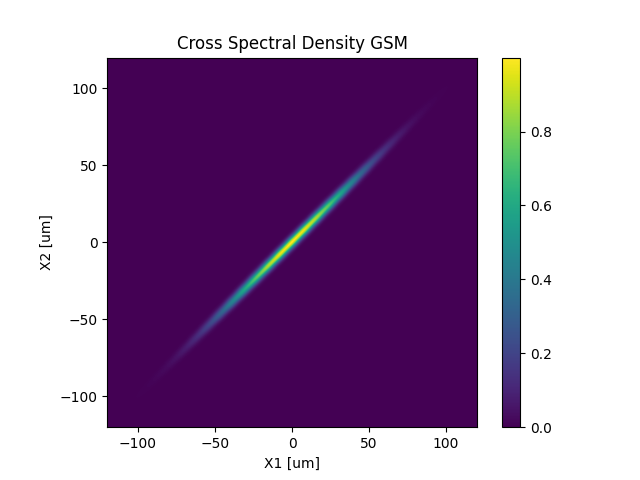
\includegraphics[width=0.49\textwidth]{figures/comparison_H_CSD_GSM.png}
    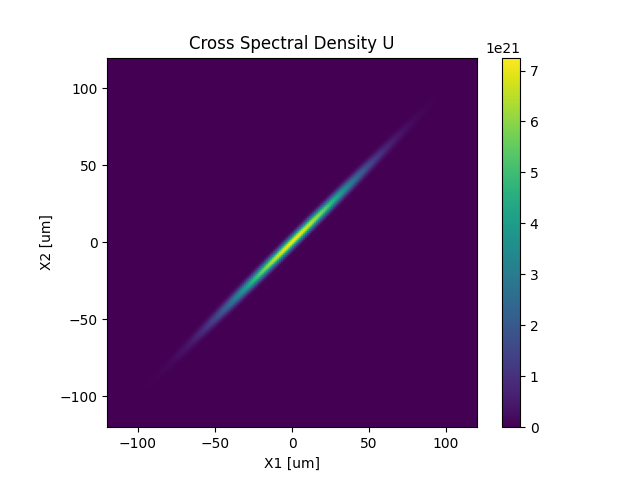
\includegraphics[width=0.49\textwidth]{figures/comparison_H_CSD_U.png}
    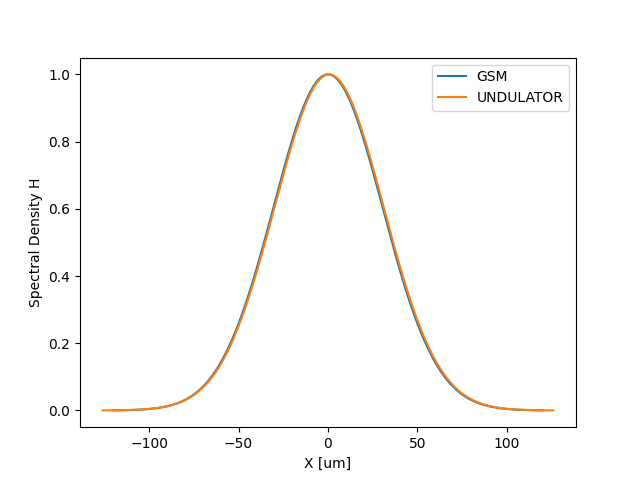
\includegraphics[width=0.59\textwidth]{figures/comparison_H_SD.png}
    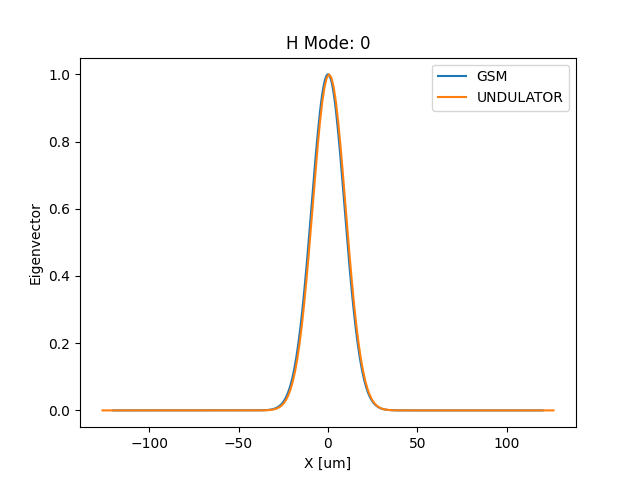
\includegraphics[width=0.49\textwidth]{figures/comparison_H_eigenvector0.png}
    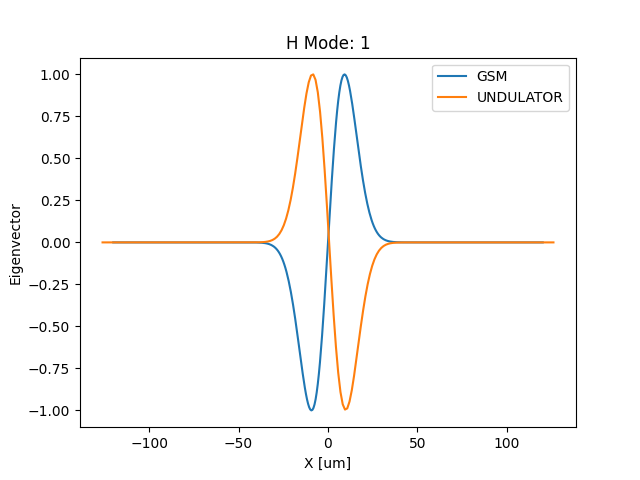
\includegraphics[width=0.49\textwidth]{figures/comparison_H_eigenvector1.png}
    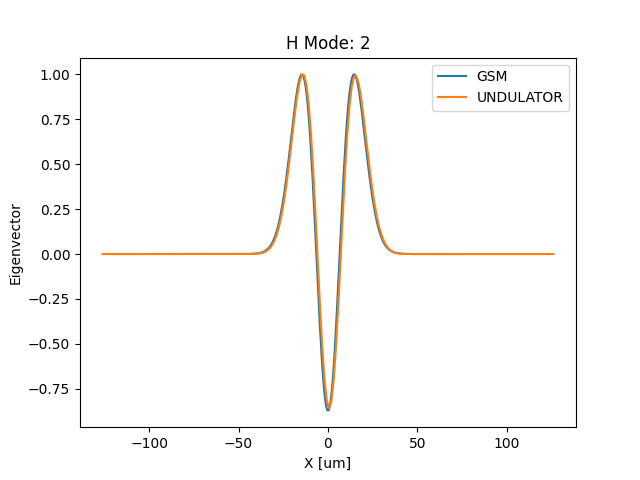
\includegraphics[width=0.49\textwidth]{figures/comparison_H_eigenvector2.png}
    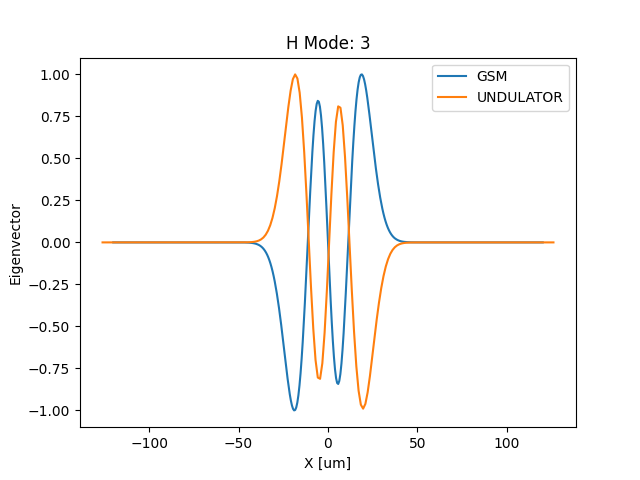
\includegraphics[width=0.49\textwidth]{figures/comparison_H_eigenvector3.png}
        
    \caption{Comparison of the approximated (GSM) and exact (1D WOFRY) coherent mode decomposition  for the Horizontal direction of a U20 undulator of length \SI{2}{\meter},  set to resonance at 10 keV photon. energy. The plot show the Cross Spectral Deisity, Spectral Density, and four first modes. The Coherence Fraction is 0.088}
    \label{fig:GSMvsUND-H}
\end{figure}


\begin{figure}
    \centering
    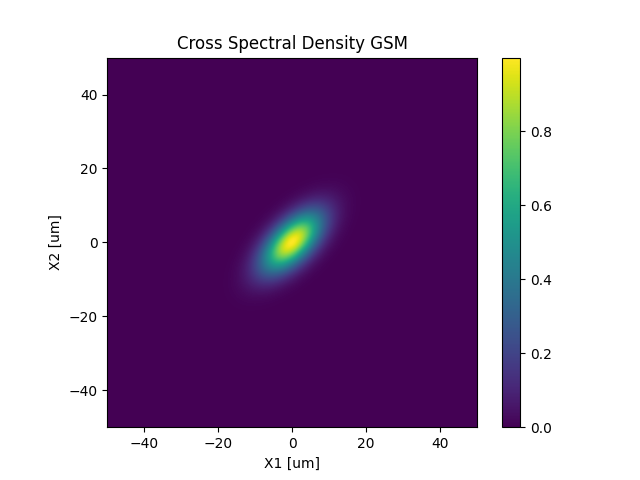
\includegraphics[width=0.49\textwidth]{figures/comparison_V_CSD_GSM.png}
    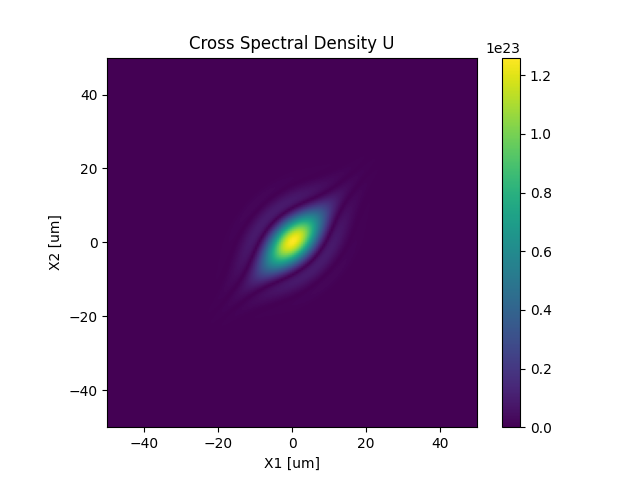
\includegraphics[width=0.49\textwidth]{figures/comparison_V_CSD_U.png}
    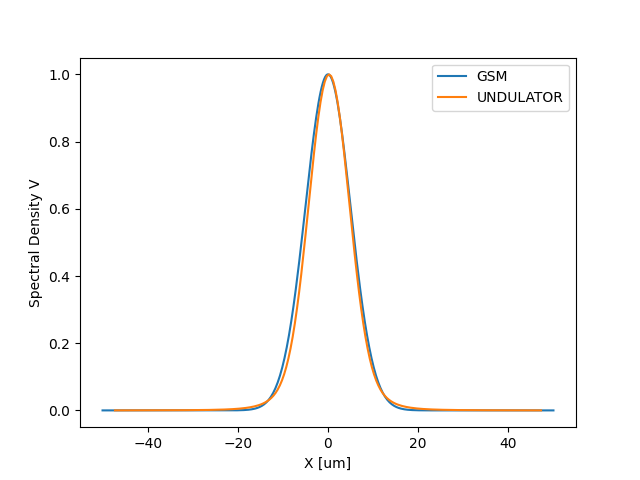
\includegraphics[width=0.59\textwidth]{figures/comparison_V_SD.png}
    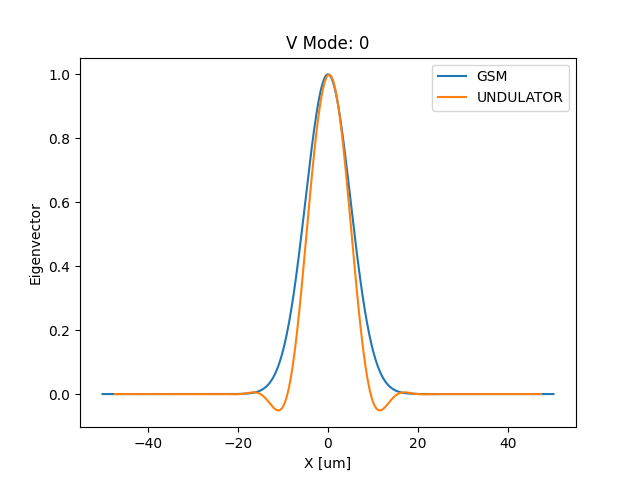
\includegraphics[width=0.49\textwidth]{figures/comparison_V_eigenvector0.png}
    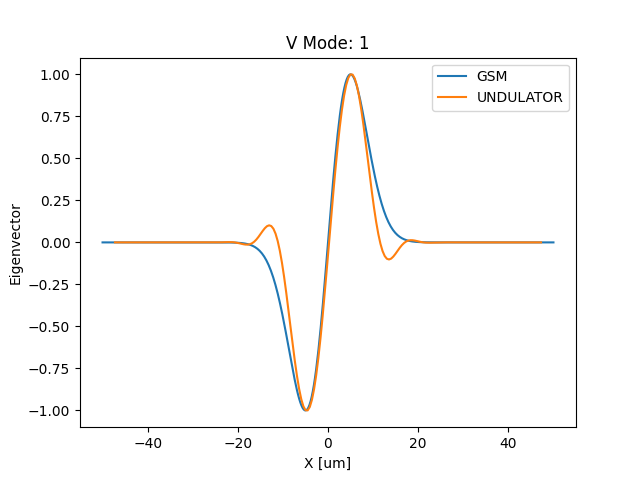
\includegraphics[width=0.49\textwidth]{figures/comparison_V_eigenvector1.png}
    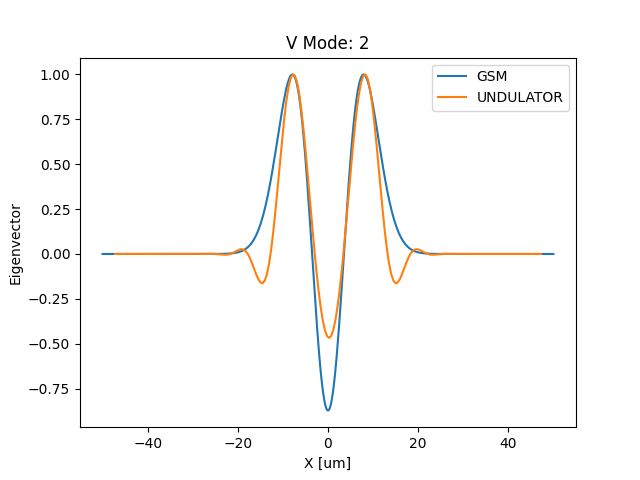
\includegraphics[width=0.49\textwidth]{figures/comparison_V_eigenvector2.png}
    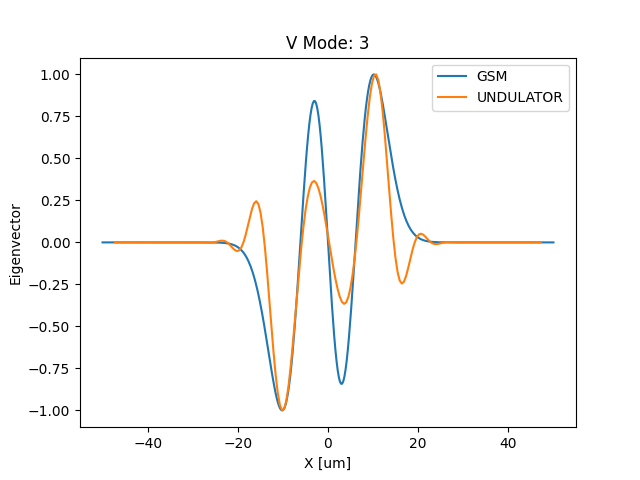
\includegraphics[width=0.49\textwidth]{figures/comparison_V_eigenvector3.png}
        
    \caption{The same as Fig.~\ref{fig:GSMvsUND-H} but for the vertical direction. The Coherence Fraction is 0.665}
    \label{fig:GSMvsUND-V}
\end{figure}



Next step is the analysis of the separability in horizontal and vertical. In Fig.~\ref{fig:GSMvsCOMSYL} we compare the coherent fraction calculated with COMSYL \cite{comsyl} and approximated by GSM (as shown in Appendix~\ref{sec:appendixA}). It shows that the GSM approximated well an undulator only for the fist modes. The Coherent Fraction (first mode) matches very well. This is due to the fact that the GSM approximation to the undulator is built matching the CF. The occupancy of higher modes differ: the first 50 GSM modes GSM to contain more than 99\% of the spectral density, but XX are needed for the numerical coherent mode decomposition with COMSYL. This means significative errors in the eigenvalues when using GSM. 

\todo{Compare COMSYL with H+V combination of WOFRY1D modes}


\begin{figure}
    \centering
    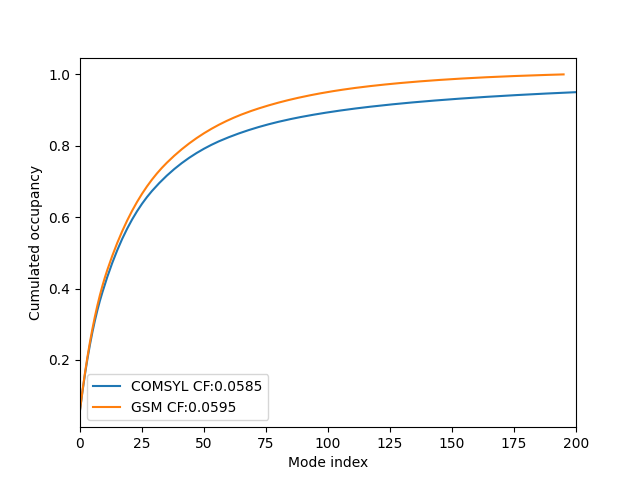
\includegraphics[width=0.95\textwidth]{figures/FigureGSMvsCOMSYL.png}
    \caption{Comparison of the approximated (GSM) and exact (COMSYL) cumulated occupation of the coherent modes for an undulator U20, of length \SI{2}{\meter}, and set to resonance at 10 keV photon. energy.}
    \label{fig:GSMvsCOMSYL}
\end{figure}

%%%%%%%%%%%%%%%%%%%%%%%%%%%%%%%%%%%%%%%%%%%%%%%%
\section{Testing the effect of a slit in the GSM}
\label{appendix:slit}

In many cases the use of the GSM supposes that during propagation over the beamline elements the beam keeps its Gaussian Shell-model nature. This is true for propagation in free space, and probably true for focusing with ideal lenses. But, in the case of slits that crop the beam, it is difficult to believe that the beam is still Gaussian. Moreover, the new beam parameters $\sigma_{I'}$ and $\sigma_{\xi'}$ are obtained supposing the slit has a width $\sigma_s$, applying
\begin{equation}
    \frac{1}{\sigma_{I'}^2} = 
    \frac{1}{\sigma_{I}^2} +
    \frac{1}{\sigma_{s}^2},
\end{equation}
and
\begin{equation}
    \sigma_{\xi'} = \sigma_{\xi} 
\end{equation}

However, there are several recipes for the relation between $\sigma_s$ and the slit aperture $A$: $\sigma_s=A/4.1$, $\sigma_s=A/2.355$ and $\sigma_s=A/\sqrt{12}$.

We have calculated the case of a Gaussian beam that is cropped by a slit. The exact calculation is compared with the GSM results using the different recipes. We have used $\sigma_x$~= \SI{30}{\micro\meter} (like for the H EBS source) and three possible values of $\beta$: quite incoherent ($\beta=0.02$), medium coherence ($\beta=0.09$) and quite coherent ($\beta=1.15$). The results are in Fig.~\ref{fig:GSMslit} where the CF is compared for the exact calculation and the GSM approximation. We remind that the CF for the GSM is $CF = 1 - q$, with $q$ given in equation~\ref{q}.
The source has been created using the GSM model with a sufficient number of modes to include more that 99\% of the spectral density. Each mode is cropped by the slit placed at the source position. The Cross Spectral Density $W$ is calculated in the usual way 
\begin{equation}
    W(x_1,x_2) = \sum \lambda_i \Phi^*(x_1) \Phi(x_2),     
\end{equation}
with $\lambda_i$ the eigenvalues of the source and $\Phi(x_{1,2})$ are the eigenvectors of the source cropped by the slit. After re-diagonalizing $W$, the new eigenvalues $\lambda_i'$ permit to calculate the exact CF: 
\begin{equation}
    CF = \frac{\lambda_0'}{\sum \lambda_i'}
\end{equation}

The results in Fig.~\ref{fig:GSMslit} show two important things:
i) the GSM model usually overestimates CF in particular for high coherence ($\beta=1.15$), where there are important discrepancies between GSM and the exact calculation.
ii) For low coherence the GSM may work, in particular when using the aperture $\sigma_s=A/2.355$, i.e., matching the Gaussian FWHM with the total aperture.

\begin{figure}
    \centering
    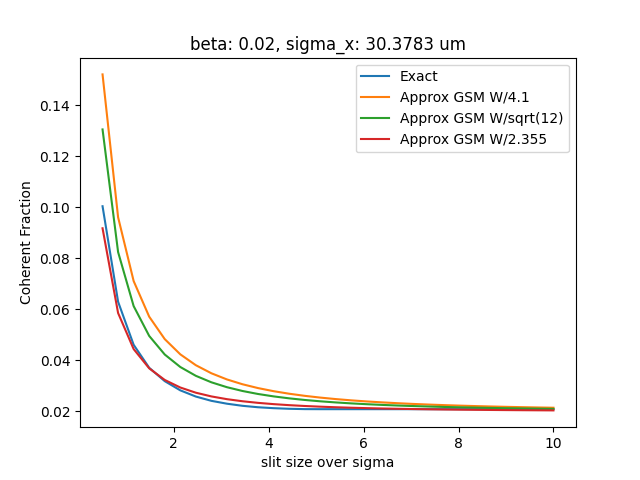
\includegraphics[width=0.95\textwidth]{figures/Figure_1a.png}
    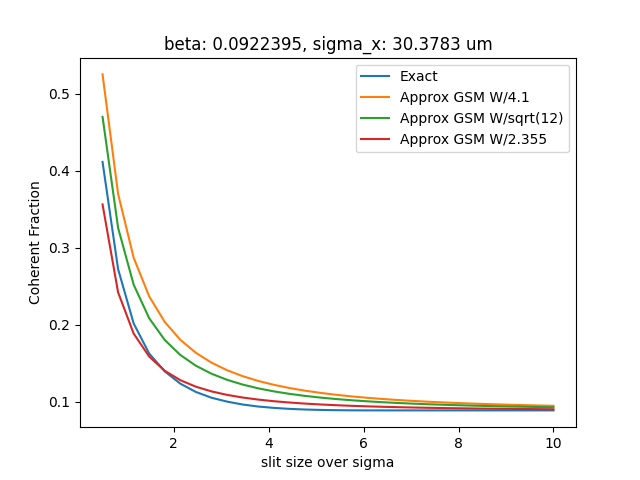
\includegraphics[width=0.95\textwidth]{figures/Figure_1b.png}
    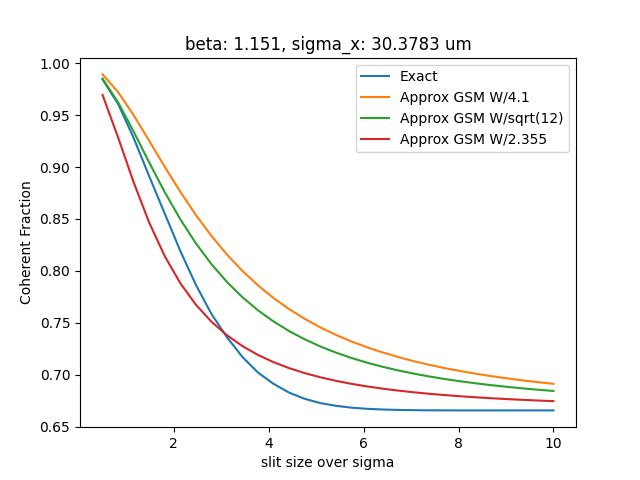
\includegraphics[width=0.95\textwidth]{figures/Figure_1c.png}
    \caption{Calculation of the coherence fraction f a Gaussian beam cropped by a slit. The exact numerical laculation (blue line) is compared with the approzimations that the beam is still described by a GSM with three possible ways to calculate the slit ``Gaussianized" $\sigma_s$ (see text). }
    \label{fig:GSMslit}
\end{figure}


% %%%%%%%%%%%%%%%%%%%%%%%%%%%%%%%%%%%%%%%%%%%%%%%%
% %%%%%%%%%%%%%%%%%%%%%%%%%%%%%%%%%%%%%%%%%%%%%%%%
% %%%%%%%%%%%%%%%%%%%%%%%%%%%%%%%%%%%%%%%%%%%%%%%%

     %-------------------------------------------------------------------------
     % The back matter of the paper - acknowledgements and references
     %-------------------------------------------------------------------------

     % Acknowledgements come after the appendices

\ack{Acknowledgements}

     % References are at the end of the document, between \begin{references}
     % and \end{references} tags. Each reference is in a \reference entry.

% \begin{references}
% \reference{Author, A. \& Author, B. (1984). \emph{Journal} \textbf{Vol}, 
% first page--last page.}
% \end{references}
% \cite{knuth84}

%% Note added by Overleaf: If using bibtex, remove the "references" environment above, and uncomment the following lines.
\bibliographystyle{iucr}
\referencelist{iucr}

     %-------------------------------------------------------------------------
     % TABLES AND FIGURES SHOULD BE INSERTED AFTER THE MAIN BODY OF THE TEXT
     %-------------------------------------------------------------------------

     % Simple tables should use the tabular environment according to this
     % model

% \begin{table}
% \caption{Caption to table}
% \begin{tabular}{llcr}      % Alignment for each cell: l=left, c=center, r=right
%  HEADING    & FOR        & EACH       & COLUMN     \\
% \hline
%  entry      & entry      & entry      & entry      \\
%  entry      & entry      & entry      & entry      \\
%  entry      & entry      & entry      & entry      \\
% \end{tabular}
% \end{table}

     % Postscript figures can be included with multiple figure blocks

% \begin{figure}
% \caption{Caption describing figure.}
% 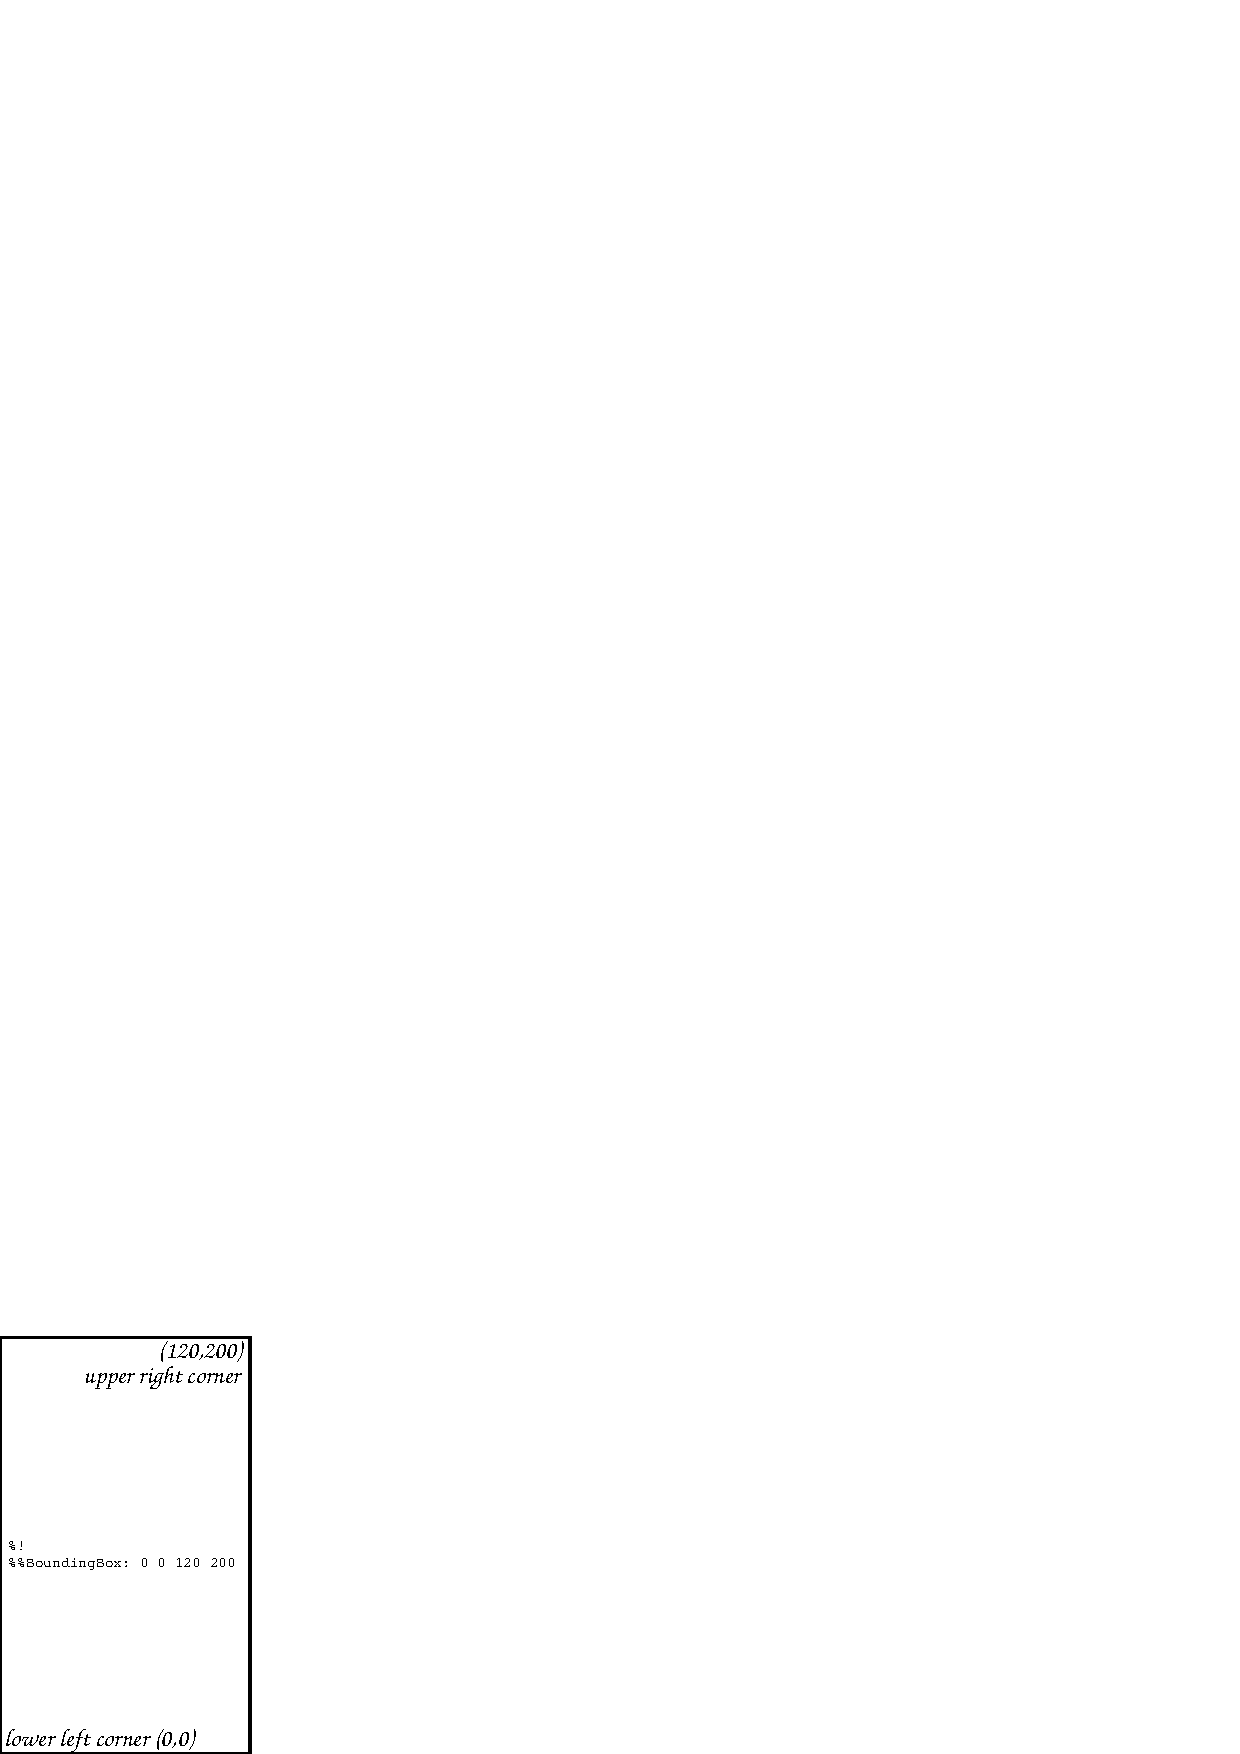
\includegraphics{fig1}
% \end{figure}


\end{document}                    % DO NOT DELETE THIS LINE
%%%%%%%%%%%%%%%%%%%%%%%%%%%%%%%%%%%%%%%%%%%%%%%%%%%%%%%%%%%%%%%%%%%%%%%%%%%%%%
